\chapter{Executor执行Task}
\section{Executor启动}

Yarn-Cluster模式下AM中SparkContext初始化完成之后,AM就开始在集群中划分资源,启动container。

AM通过循环等待spark.yarn.am.waitTime中定义的时间监听SparkContext的初始化状态,最后获得SparkContext的初始化实例。如果初始化实例为空,则报错并将应用状态置为失败。SparkContext不为空的情况下,将会注册AM。注册AM核心代码如程序\ref{inputPrg:registeram}所示
\begin{codeInput}{Scala}{Driver端am注册}{registeram}
allocator = client.register(driverUrl,
driverRef,
yarnConf,
_sparkConf,
uiAddress,
historyAddress,
securityMgr)
allocator.allocateResources()
reporterThread = launchReporterThread()
\end{codeInput}

程序\ref{inputPrg:registeram}中client其实为YarnRMClient,是与RM\footnote{RM为ResourceManager的简称,以后提到RM均为ResourceManage}负责通信的。client.register的作用就是向RM中注册AM,并获得YarnAllocator实例对象,此对象的作用体现在下一行代码。

程序的调用栈如下所示
\begin{orgianlboxnotitle}
	(1)YarnAllocator\#allocateResources()\\
	(2)YarnAllocator\#handleAllocatedContainers\\
	(3)YarnAllocator\#runAllocatedContainers
\end{orgianlboxnotitle}

调用栈(1)负责和RM通信确保资源能够满足请求的资源,如果满足将会生成和请求资源最大Executor数量相等的Container。调用栈(2)将会匹配RM所提供的Container,并决定在其上启动Executor。调用栈(3)是负责启动的模块,也是本程序的重点,其代码段如程序\ref{inputPrg:runContainer}所示,流程图如图\ref{fig:runContainer}所示。
\begin{figure}[H] 
	\centering
	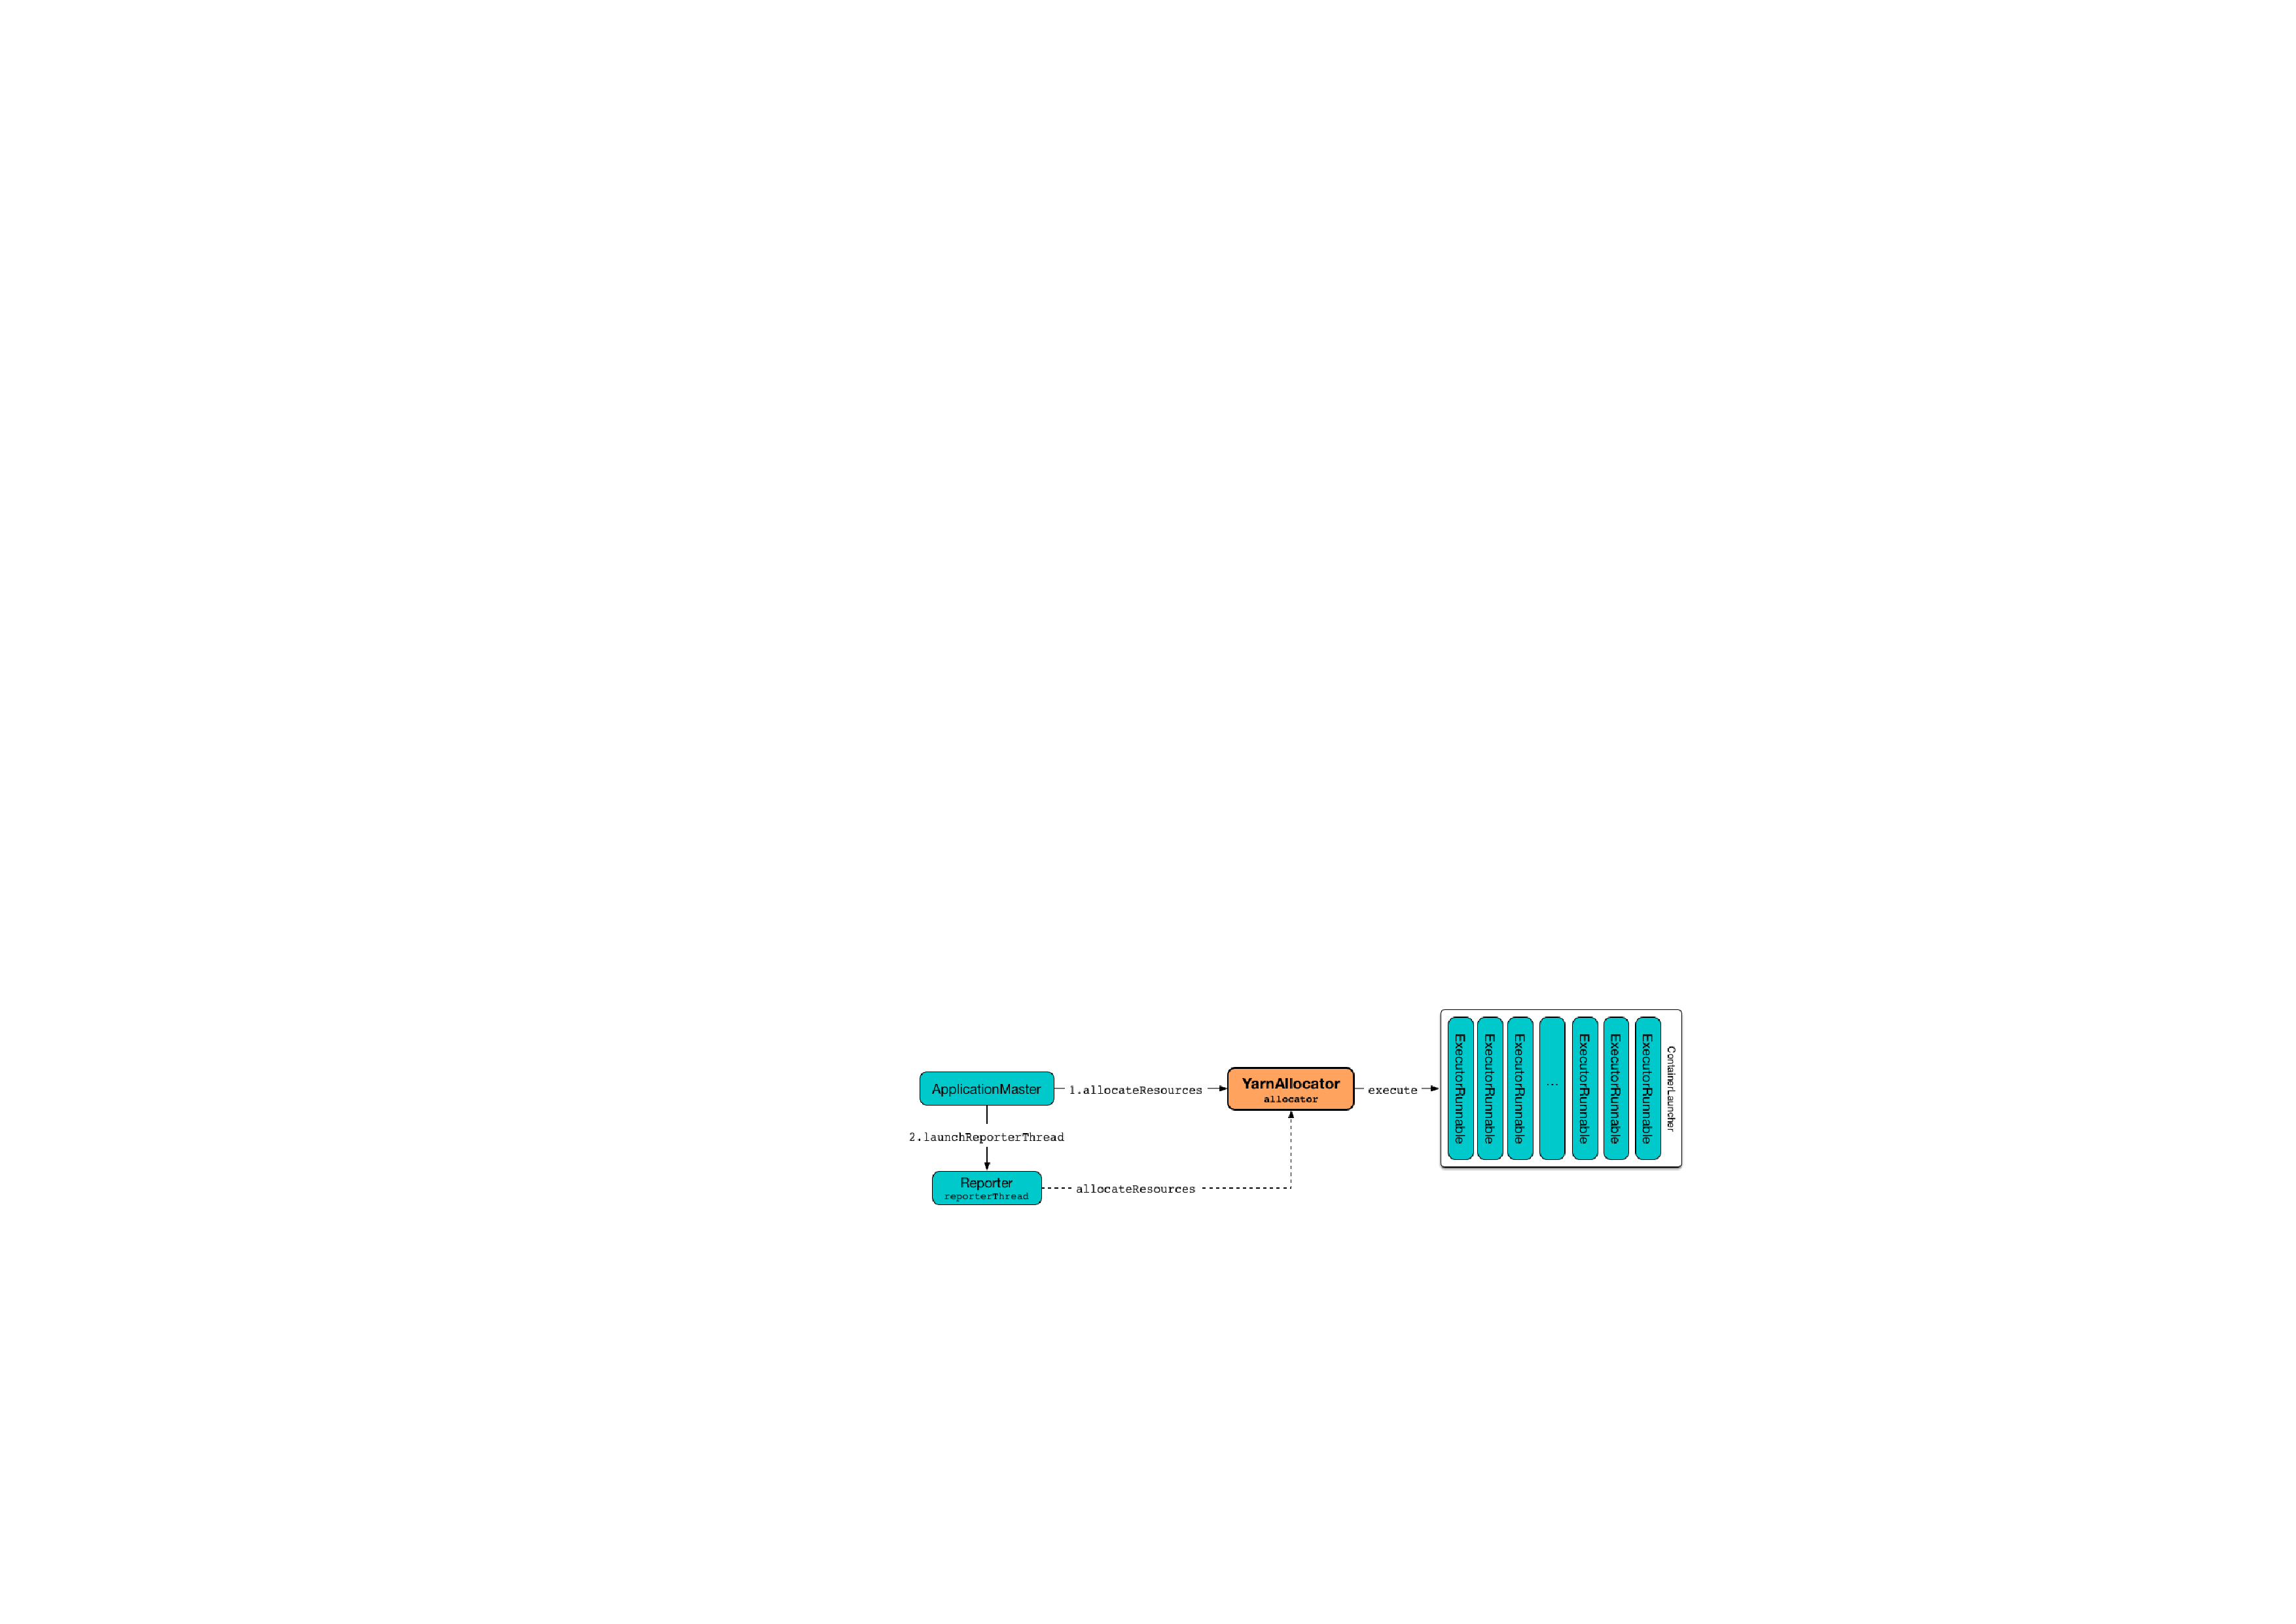
\includegraphics[width=\textwidth]{figures/YarnAllocator.pdf}
	\caption{YarnAllocator启动Container流程}
	\label{fig:runContainer}
\end{figure}
\begin{codeInput}{Scala}{启动Executor}{runContainer}
for (container <- containersToUse) {
  numExecutorsRunning += 1
  val executorHostname = container.getNodeId.getHost
  val containerId = container.getId
  executorIdCounter += 1
  val executorId = executorIdCounter.toString
  executorIdToContainer(executorId) = container
  containerIdToExecutorId(container.getId) = executorId	
  val containerSet = allocatedHostToContainersMap.getOrElseUpdate(executorHostname,
    new HashSet[ContainerId])	
  containerSet += containerId
  allocatedContainerToHostMap.put(containerId, executorHostname)	
  val executorRunnable = new ExecutorRunnable(container,conf,sparkConf,driverUrl,executorId,
  executorHostname,executorMemory,executorCores,
  appAttemptId.getApplicationId.toString,securityMgr)
  if (launchContainers) {
    launcherPool.execute(executorRunnable)
  }
}
\end{codeInput}

targetNumExecutors为Executor的总数,默认情况为2,当用户没有开启动态分配并手动指定targetNumExecutors的数量时,系统会逐个Executor分配Container。同时会将生成的Executor标识唯一的ID,且与Container进行绑定,最后会通过ExecutorRunnable实例的run方法到NM\footnote{NM为NodeManager的简称,以后提到NM均为NodeManage}中启动Container。每个Container中包含了Executor的核数和内存大小,通过Java命令启动Executor实例即CoarseGrainedExecutorBackend。CoarseGrainedExecutorBackend的main方法首先会对启动它时传来的参数进行解析,只会会调用run方法,代码细节如程序\ref{inputPrg:executorBackendRun}所示
\begin{codeInput}{Scala}{CoarseGrainedExecutorBackend.run}{executorBackendRun}
SignalLogger.register(log)
SparkHadoopUtil.get.runAsSparkUser { () =>
  val executorConf = new SparkConf
  val port = executorConf.getInt("spark.executor.port", 0)
  //这个fetcher通过rpcenv用来获得driver的ref,之后就关闭了
  val fetcher = RpcEnv.create("driverPropsFetcher",hostname,port,
  executorConf,new SecurityManager(executorConf),clientMode = true)
  val driver = fetcher.setupEndpointRefByURI(driverUrl)
  //获得Driver端的配置信息
  val props = driver.askWithRetry[Seq[(String, String)]](RetrieveSparkProps) ++
  Seq[(String, String)](("spark.app.id", appId))
  fetcher.shutdown()	
  // 使用从Driver端获取的配置信息创建SparkEnv
  val driverConf = new SparkConf()
    for ((key, value) <- props) {
      if (SparkConf.isExecutorStartupConf(key)) {
        driverConf.setIfMissing(key, value)
      } else {
        driverConf.set(key, value)
      }
    }
  //这里如果是yarn模式下,他其实一直在跟新和HDFS交互的密钥信息
  if (driverConf.contains("spark.yarn.credentials.file")) {
    SparkHadoopUtil.get.startExecutorDelegationTokenRenewer(driverConf)
  }
  //创建ExecutorEnv,代码和Driver端的基本一摸一样
  val env = SparkEnv.createExecutorEnv(driverConf, executorId, hostname, port, cores, isLocal = false)	
  val sparkHostPort = env.conf.getOption("spark.executor.port").map { port =>
    hostname + ":" + port}.orNull
  //这里创建了一个Endpoint用于与driver交互执行task。是由此可以看出Executor的真正实现CoarseGrainedExecutorBackend
  env.rpcEnv.setupEndpoint("Executor", new CoarseGrainedExecutorBackend(
  env.rpcEnv, driverUrl, executorId, sparkHostPort, cores, userClassPath, env))
  //WorkerWatcher就是用来监视worker的,当与worker断开连接时,它将会关闭这个jvm进程
  workerUrl.foreach { url =>
    env.rpcEnv.setupEndpoint("WorkerWatcher", new WorkerWatcher(env.rpcEnv, url))
  }
  env.rpcEnv.awaitTermination()
  SparkHadoopUtil.get.stopExecutorDelegationTokenRenewer()
}
\end{codeInput}

Executor创建于Driver交互的RPC环境后,会立刻执行CoarseGrainedExecutorBackend的onStart()方法,该方法最重要的作用是向Driver注册Executor的信息,主要为executorId和cores等。注册的消息会在CoarseGrainedSchedulerBackend\#receiveAndReply中接收,在Driver端会通过executorDataMap(HashMap[String,ExecutorData])数据结构进行存储,TaskScheduler对将task封装为TaskDescription时会用到executorDataMap中的信息。
\section{Task的执行}

第\ref{jobrunning}章Driver通过CoarseGrainedSchedulerBackend.DriverEndPoint.launchTasks会将Task分配到Executor上,这里通过的是nettyRpc。

CoarseGrainedExecutorBackend收到LaunchTask消息后,会调用Executor的launchTask启动Task,如程序\ref{inputPrg:executorlaunchtask}
\begin{codeInput}{Scala}{CoarseGrainedExecutorBackend消息处理模块}{executorlaunchtask}
case LaunchTask(data) =>
  if (executor == null) {
    logError("Received LaunchTask command but executor was null")
    System.exit(1)
  } else {
    val taskDesc = ser.deserialize[TaskDescription](data.value)
    logInfo("Got assigned task " + taskDesc.taskId)
    executor.launchTask(this, taskId = taskDesc.taskId, attemptNumber = taskDesc.attemptNumber,
    taskDesc.name, taskDesc.serializedTask)
}
\end{codeInput}

Executor.launchTask方法如程序块\ref{inputPrg:executorrunner}所示
\begin{codeInput}{Scala}{Executor.launcherTask}{executorrunner}
val tr = new TaskRunner(context, taskId = taskId, attemptNumber = attemptNumber, taskName,
serializedTask)
runningTasks.put(taskId, tr)
threadPool.execute(tr)
\end{codeInput}

Executor会输入的Task生成一个TaskRunner,最终会被放到一个ThreadPool中去。TaskRunner为一个线程,重写其run方法,run中会执行Task。

\subsection{Task执行前的准备}

Driver端生成Task的时候会将Task依赖的文件和jar信息都封装到Task中去,在Executor端,得先恢复这些信息。
\begin{orgianlboxnotitle}
  val (taskFiles,taskJars,taskBytes) = Task.deserializeWithDependencies(serializedTask)\\
  updateDependencies(taskFiles, taskJars)
\end{orgianlboxnotitle}

这里返回了三元组,信息包含了taskFiles、taskJars和taskBytes,这些信息只是属于类似于元数据的信息,接下来Executor还需要调用updateDependencies下载这些依赖:
\begin{orgianlboxnotitle}
// Fetch file with useCache mode, close cache for local mode.\\
Utils.fetchFile(name, new File(SparkFiles.getRootDirectory()), conf,\\
env.securityManager, hadoopConf, timestamp, useCache = !isLocal)
\end{orgianlboxnotitle}

依赖下载完成后,Executor会通过TaskRunner来执行Task。
\subsection{执行Task}

准备工作做好后,Executor就是执行Task.run方法来运行Task,如程序\ref{inputPrg:executorruntask}所示
\begin{codeInput}{Scala}{Execotor执行Task}{executorruntask}
//开始执行Task
taskStart = System.currentTimeMillis()
var threwException = true
val (value, accumUpdates) = try {
  val res = task.run(
  taskAttemptId = taskId,
  attemptNumber = attemptNumber,
  metricsSystem = env.metricsSystem)
  threwException = false
  res
} finally {
  ......
}
val taskFinish = System.currentTimeMillis()
\end{codeInput}

程序\ref{inputPrg:executorruntask}中task.runTask会调用Task.run方法,此方法为final类型,首先会本次Task生成TaskContext,也就是保留本Task的上下文信息。最后TaskContext还会在Task执行完成后对次Task标记成功并通过回调函数来完成最终的处理,如程序\ref{inputPrg:marktaskcomplete}所示
\begin{codeInput}{Scala}{TaskContext任务成功时执行回调}{marktaskcomplete}
private[spark] def markTaskCompleted(): Unit = {
  completed = true
  val errorMsgs = new ArrayBuffer[String](2)
  onCompleteCallbacks.reverse.foreach { listener =>
  try {
    listener.onTaskCompletion(this)
  } catch {
    case e: Throwable =>
      errorMsgs += e.getMessage
    }
  }
  if (errorMsgs.nonEmpty) {
    throw new TaskCompletionListenerException(errorMsgs)
  }
}
\end{codeInput}

整个Task.run的核心程序如\ref{inputPrg:taskrun}所示
\begin{codeInput}{Scala}{Task run方法核心部分}{taskrun}
//设置上下文信息,实际上会调用org.apache.spark.TaskContext#setTaskContext
TaskContext.setTaskContext(context)
//更新metrics信息
context.taskMetrics.setHostname(Utils.localHostName())
context.taskMetrics.setAccumulatorsUpdater(context.collectInternalAccumulators)
//当前线程,在被打断的时候可以通过它来停止该线程
taskThread = Thread.currentThread()
if (_killed) {//如果当前Task被杀死,那么需要退出Task的执行
  kill(interruptThread = false)
}
try {
  //执行本次Task,runTask真正执行代码为子类中重写的runTask,对应ShuffleMapTask和ResultTask
  (runTask(context), context.collectAccumulators())
} catch {
} finally {
  // Call the task completion callbacks.
  context.markTaskCompleted()
  try {
  }
  } finally {
    TaskContext.unset()
  }
}
\end{codeInput}

这里的runTask会有两种不同的实现方法,分别为ShuffleMapTask和ResultTask,两种Task前期阶段处理基本相同,如程序\ref{inputPrg:common}所示。
\begin{codeInput}{Scala}{两种Task共同的处理方式}{common}
// Deserialize the RDD using the broadcast variable.
val deserializeStartTime = System.currentTimeMillis()
//获取反序列化实例
val ser = SparkEnv.get.closureSerializer.newInstance()
//以下两端代码是其区别,上面的为ShuffleMapTask,下面为ResultTask
val (rdd, dep) = ser.deserialize[(RDD[_], ShuffleDependency[_, _, _])](
//获取rdd和作用于rdd结果的函数
val (rdd, func) = ser.deserialize[(RDD[T], (TaskContext, Iterator[T]) => U)](

ByteBuffer.wrap(taskBinary.value), Thread.currentThread.getContextClassLoader)
_executorDeserializeTime = System.currentTimeMillis() - deserializeStartTime
//Task的测量信息
metrics = Some(context.taskMetrics)
\end{codeInput}
\begin{enumerate}[\bfseries 1]
	\item 对于ShuffleMapTask
	
	ShuffleMapTask是根据Stage中分区数量来生成的,它会根据该Stage每个RDD连接操作作用于对应的partition上,并将结果生成文件供下游Task使用。ShuffleMapTask核心代码段如程序\ref{inputPrg:shufflemaptask}所示
\begin{codeInput}{Scala}{ShuffleMapTask核心部分实现分析}{shufflemaptask}
//从SparkEnv中获得shuffleManager,具体分析会在shuffle模块讲述
val manager = SparkEnv.get.shuffleManager
//从shuffleManager获得写入器
writer = manager.getWriter[Any, Any](dep.shuffleHandle, partitionId, context)
//调用rdd开始计算,并且最后通过写入器写入文件系统
writer.write(rdd.iterator(partition, context).asInstanceOf[Iterator[_ <: Product2[Any, Any]]])
//关闭写入器,并将最后结果返回
writer.stop(success = true).get
\end{codeInput}
	\item 对于ResultTask
	
	ResultStage会根据生成结果的Partition来生成与Partition数量相同的ResultTask,最后会将计算结果回传给Driver端,这里的结果不一定是真实的数据。ResultTask的作用代码如程序\ref{inputPrg:ResultTask}所示。
\begin{codeInput}{Scala}{ResultTask核心部分实现分析}{ResultTask}
//调用rdd的迭代器执行传入函数的操作
func(context, rdd.iterator(partition, context))
\end{codeInput}
\end{enumerate}

\subsection{Task结果的处理}
Executor运行完Task后,就会将结果保存在DirectTaskResult里,如程序\ref{inputPrg:executorresult}所示
\begin{codeInput}{Scala}{Executor对Task结果的处理}{executorresult}
//任务运行结果的处理
val resultSer = env.serializer.newInstance()
val beforeSerialization = System.currentTimeMillis()
//value中保存Task的计算结果
val valueBytes = resultSer.serialize(value)
val afterSerialization = System.currentTimeMillis()
//首先将结果直接放入org.apache.spark.scheduler.DirectTaskResult
val directResult = new DirectTaskResult(valueBytes, accumUpdates, task.metrics.orNull)
val serializedDirectResult = ser.serialize(directResult)
val resultSize = serializedDirectResult.limit
\end{codeInput}

但是serializedDirectResult并不是直接回传给Driver,Executor通过程序\ref{inputPrg:executorsendresult}的策略对结果进行不同处理。
\begin{codeInput}{Scala}{Executor回传结果策略}{executorsendresult}
// directSend = sending directly back to the driver
val serializedResult: ByteBuffer = {
if (maxResultSize > 0 && resultSize > maxResultSize) {
  //如果resultSize大于spark.drive.driver.maxResultSize设置的大小值,则直接丢弃
  ser.serialize(new IndirectTaskResult[Any](TaskResultBlockId(taskId), resultSize))
} else if (resultSize >= akkaFrameSize - AkkaUtils.reservedSizeBytes) {
  //如果不能通过AKKA的消息传递,那么放入BlockManager等待调用者以网络形式来获取
  //AKKA的消息默认大小可以通过spark.akka.frameSize来设置
  val blockId = TaskResultBlockId(taskId)
  env.blockManager.putBytes(
  blockId, serializedDirectResult, StorageLevel.MEMORY_AND_DISK_SER)
  ser.serialize(new IndirectTaskResult[Any](blockId, resultSize))
} else {
  //结果回传Driver
  serializedDirectResult
 }
}
//通过AKKA向driver汇报本次Task已经完成
execBackend.statusUpdate(taskId, TaskState.FINISHED, serializedResult)
\end{codeInput}

而execBackend.statusUpdate实际上调用的CoarseGrainedExecutorBackend.statusUpdate,程序如\ref{inputPrg:execbankendstatus}所示
\begin{codeInput}{Scala}{Executor执行回传消息}{execbankendstatus}
val msg = StatusUpdate(executorId, taskId, state, data)
driver match {
  case Some(driverRef) => driverRef.send(msg)
  case None => logWarning(s"Drop $msg because has not yet connected to driver")
}
\end{codeInput}

这里通过DriverRef通过Rpc机制实际会调用TaskschedulerImpl.statusUpdate。Driver端对结果的处理见小节\ref{driverdealresult}。
\section{Executor生命周期}
本章主要介绍Executor启动的过程、Task的分发、Task的运行以及Executor对Task结果的处理。Executor运行Task这个过程的时序图如图\ref{fig:ExecutorRunTask}所示
\begin{figure}[H] 
\centering
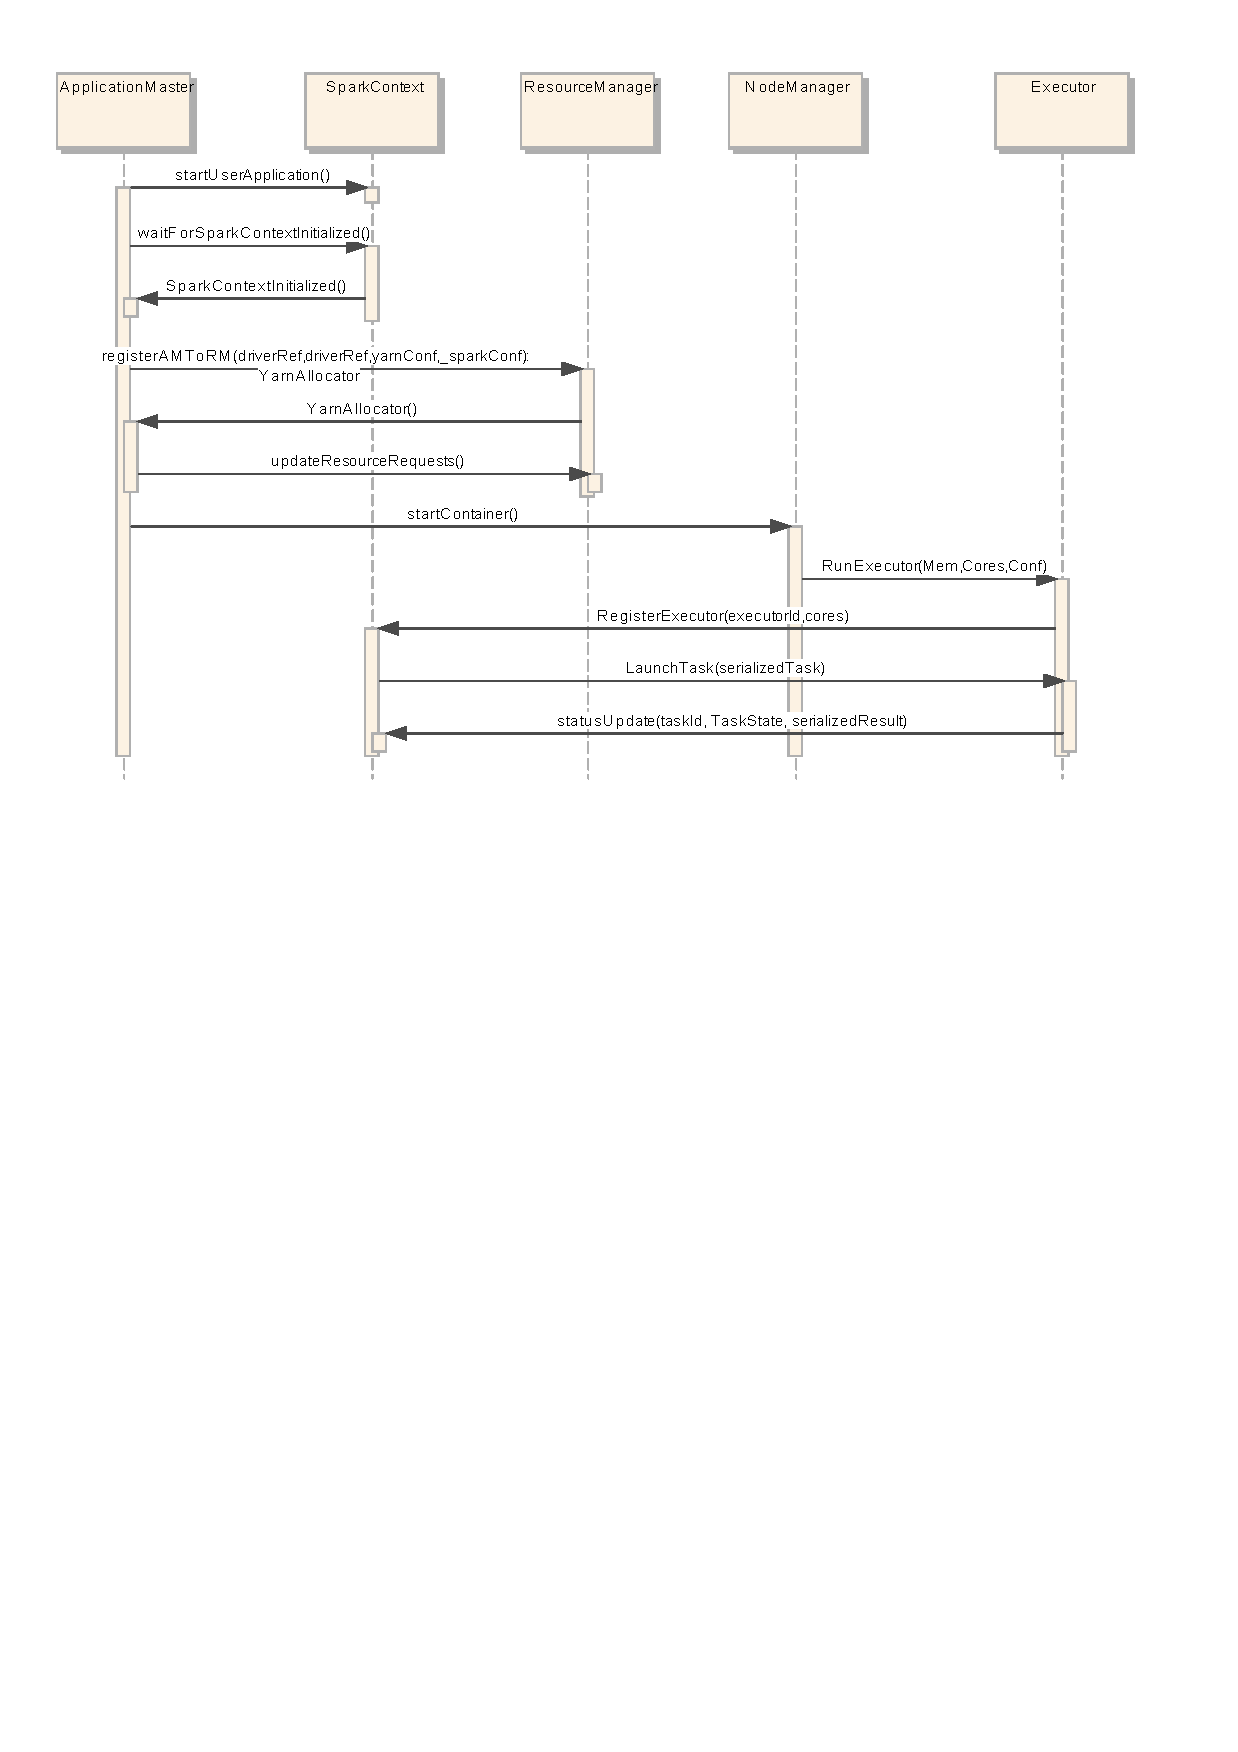
\includegraphics[width=\textwidth]{figures/ExecutorRunTask.pdf}
\caption{Executor运行Task时序图}
\label{fig:ExecutorRunTask}
\end{figure}